% !TeX spellcheck = en_GB

\cleardoublepage
% ***************************************************** %
\section{Experiments and results discussion}\label{sc:exp}
% ***************************************************** %

To test the efficiency the algorithms, a benchmark of six datasets retrieved from \href{https://www.csie.ntu.edu.tw/~cjlin/libsvmtools/datasets/}{LIBSVM} is used, see table~\vref{tab:datasets} for details. Every dataset comes already pre-processed, with every sample scaled in range $[-1,1]$ and the response variable in $\set{-1,1}$; many features are categorical with values $0,1,2\dots$, this implies that the dataset matrix can be stored in sparse format, so the \texttt{SciPy} CSR matrix format was used.

Compared to the available benchmark dataset, those chosen are not that large, the choice is due to the hardware available (Intel\textregistered\xspace Core\texttrademark\xspace i\num{7}, memory \mbox{\num{16}GB}). As can be seen few dataset are unbalanced, this will affect the accuracy.%\par\smallskip

\subsection{Solving the optimization problem}

%The regularization coefficient from~\eqref{eq:opt-prob} is set to $\lambda=0.5$ and the tolerance from the stopping criterion~\eqref{eq:stopping} $\epsilon=\num{e-3}$; the momentum term $\beta_0=0.9$, the aggressiveness of the Armijo condition is set to a small value $\gamma=\num{e-3}$; and regarding failures for exceeding epochs and iterations $k^\ast=600$ and $q^\ast=100$ for both Armijo method and momentum correction.
In order to solve the optimization problem, an initial guess $w^0$ for the model weights is given: we set a null \emph{bias} and the other features are drawn from an uniform distribution in range $[-0.5,0.5]$.

Then a \emph{hyper-parameters tuning} is performed. We set fixed values for the $\lambda$ regularization coefficient from~\eqref{eq:opt-prob}, the $\epsilon$ tolerance from the stopping criterion~\eqref{eq:stopping}, the initial momentum term $\beta_0$ and the aggressiveness of the Armijo condition $\gamma$ to a small value. Regarding failures for exceeding epochs and iterations, $k^\ast$ and $q^\ast$ for both Armijo method and momentum correction were set. Follow the values
\[
\begin{array}{lll}
\toprule
\lambda=0.5 & \epsilon=\num{e-3} & \beta_0=0.9 \\
\gamma=\num{e-3} & k^\ast=600 & q^\ast=100 \\
\bottomrule
\end{array}
\]

Moving to the other hyper-parameters, a \emph{grid search}, without cross-validation but just using test data for comparison, is applied to find the best combination for each algorithm. The procedure confronts different combinations of the mini-batch size, the learning rate in the basic SGD version and the ones with line search, and in the latter are confronted also different values for the damping both in the Armijo method and momentum correction.

The mini-batch size grid depends on the dataset being considered. As said, the retrieved datasets vary in size, but the general rule is to stay around 100 iterations using values that are powers of 2, the grid is composed by at least two values. For the first five datasets, the size starts at 32. Follows the grids used
%\begin{center}
%\begin{tabular}{lll}
%\toprule
%%Hyper-parameter & Algorithm & Values \\
%%\midrule
%$M$ & \texttt{SGD-}, \texttt{SGDM-} & depends on dataset \\
%$\alpha_0$ & \texttt{SGD-Fixed}, \texttt{SGDM} & \numlist{1; 0.5; 0.1; 0.01; 0.001; 0.0005} \\
%$\alpha_0$ & \texttt{SGD-Decreasing} & \numlist{1; 0.8; 0.5; 0.1; 0.05; 0.01; 0.005} \\
%$\alpha_0$ & \texttt{SGD-Armijo}, \texttt{MSL-SGDM-C/R} & \numlist{1; 0.5; 0.1; 0.05; 0.01; 0.005} \\
%$\delta_a$ & \texttt{SGD-Armijo}, \texttt{MSL-SGDM-C/R} & \numlist{0.3; 0.5; 0.7; 0.9} \\
%$\delta_m$ & \texttt{MSL-SGDM-C} & \numlist{0.3; 0.5; 0.7} \\
%\bottomrule
%\end{tabular}\par\noindent
%\end{center}
\[
\begin{array}{lll}
\toprule
\alpha_0 & \text{\texttt{SGD-Fixed}}, \text{\texttt{SGDM}} & \numlist{1; 0.5; 0.1; 0.05; 0.01; 0.005; 0.001} \\
\alpha_0 & \text{\texttt{SGD-Decreasing}} & \numlist{1; 0.8; 0.5; 0.1; 0.05; 0.01; 0.005} \\
\alpha_0 & \text{\texttt{SGD-Armijo}}, \text{\texttt{MSL-SGDM-C/R}} & \numlist{1; 0.5; 0.1; 0.05; 0.01; 0.005} \\
M & \text{\texttt{SGD-}}, \text{\texttt{SGDM-}} & \text{depends on dataset} \\
\delta_a & \text{\texttt{SGD-Armijo}}, \text{\texttt{MSL-SGDM-C/R}} & \numlist{0.3;0.5;0.7} \\
\delta_m & \text{\texttt{MSL-SGDM-C}} & \numlist{0.3; 0.5; 0.7} \\
\bottomrule
\end{array}
\]
where $\delta_a$ is the damping for the Armijo line search and $\delta_m$ for the momentum correction, the combinations for the \texttt{MSL-SGDM-C} are three times those of \texttt{SGD-Armijo} and \texttt{MSL-SGDM-R}.

As you can see, the upper-bound for the step-size is limited to \num{1}, this because, as the grid search pointed out then, the algorithms perform better with a smaller step-size. Therefore, on each epoch the line search will spend time reducing the initial learning rate, while the basic versions, \texttt{SGD-Fixed} and \text{SGDM}, will end up far from the solution.

The grid search chooses the best combination for a certain solver based on the greatest \emph{test accuracy} and lowest \emph{objective function} value. The results can be seen in tables from~\vref{tab:w1a-table} to~\ref{tab:a4a-tab} ordered descending by accuracy on the test dataset and ascending by objective function on reached solution. The other displayed values are the number of epochs and the run-time, the solution norm and the gradient norm.

For benchmarking purposes the optimization problem is solved also using the \texttt{Full-batch Gradient Descent} and three solvers from \texttt{SciPy} which are \texttt{L-BFGS}, \texttt{Conjugate Gradient} and \texttt{Newton-CG}.%\par\smallskip

Regarding the grid search implementation, the \texttt{Joblib} module was used to parallelize on multiple cores the \texttt{for loop} needed to evaluate the algorithm with various combinations, see algorithm~\vref{alg:grid-search}.\par\smallskip

%Speaking of the results, the algorithms that use the line search obviously take more time to terminate
%struggle to reach the $\epsilon$ tolerance

%Per quanto riguarda gli algoritmi che fanno uso della line search, per prima cosa si nota che ovviamente il loro tempo di esecuzione è maggiore degli altri; in ogni dataset si nota la loro difficoltà nel raggiungere la $\epsilon$ tolerance nonostante il limite di 600 epoche. Bisogna comunque tener presente che nel machine learning non è richiesto di arrivare ad una precisione estremamente bassa.

%Il metodo col full-batch per queste dimensioni del dataset si dimostra una scelta valida, anche perché nel caso della regressione logistica è possibile calcolare il gradiente in forma chiusa come visto, stessa cosa per i solver di \texttt{SciPy}, inoltre questi avendo condizioni d'arresto diverse arrivano ad una tolleranza ancora più inferiore, che come detto non è richiesta nel machine learning.

%Come ci si aspettava, l'accuracy è molto influenzata dallo sbilanciamento del dataset, per questo fenomeno si potrebbe ricorrere all'uso di metriche diverse. In tutti i casi i valori non sono molto distanti tra un solver e l'altro.

% il full-batch è sempre migliore della versione mini-batch nel fixed

%Thanks to the $\ell_2\text{-regularization}$ the algorithm searches for near the null model

First thing to say, the regularization term has a great influence on the final model, as you can see in the solution norm column the values are not that high, %however lowering the $\lambda$ coefficient would have led to a smaller solution norm, so the null model, possibly when the stochastic line search is used.
lowering the $\lambda$ coefficient would lead to a lower objective function value, should be seen the change in the solution norm.

Speaking of the algorithms that use the Armijo line search, first of all one notices that their execution time is obviously longer than the others. More important, in each dataset you can see that the $\epsilon$ tolerance value is never reached though the limit of 600 epochs, especially the \texttt{SGD-Armijo} algorithm. However, in machine learning a very low tolerance is not necessarily required. Nonetheless the SLS solvers prove to achieve a higher accuracy, particularly the \texttt{SGD-Armijo}.

The full-batch method for these dataset sizes is still a valid choice and could reach also a lower tolerance value, most of all has the lower run-time among the SGD solvers, followed by the \texttt{SGD-Decreasing}. Same for the \texttt{scipy.optimize} solvers that can reach the smallest gradient norm. The \texttt{Mushrooms} dataset is an exception, where these solvers converge to the lowest solution norm with the lowest accuracy.

As expected the accuracy is greatly influenced by the class distribution of each datasets, for which different metrics that deal with unbalanced datasets could be used. Between al solvers the test score is very similar, as the $f(w^\ast)$ except in some cases for the \texttt{SGD-Armijo} solver that ended on a different solution with even higher accuracy.

\subsection{Performance of the objective function}

Now, as done by the authors of both articles, we want to show how the value of the objective function decreases with each epoch and also during time. For this purpose, another \emph{grid search} is performed, again the fixed hyper-parameters are
%We set $k^\ast=200$ and run the algorithms with the best hyper-parameters from the grid search, but varying the learning rate in grid \numlist{1; 0.1; 0.01}. Results can be seen in figures from~\vref{fig:w1a-w3a} to~\ref{fig:mush-a4a}.
\[
\begin{array}{lll}
\toprule
\lambda=0.5 & \epsilon=\num{e-3} & \beta_0=0.9 \\
\gamma=\num{e-3} & k^\ast=200 & q^\ast=100 \\
\bottomrule
\end{array}
\]

What differs now is that the grid search finds the best hyper-parameters for each learning rate in \numlist{1; 0.1; 0.01}, hence the grids are
%\begin{center}
%\begin{tabular}{lll}
%\toprule
%%Hyper-parameter & Algorithm & Values \\
%%\midrule
%$M$ & \texttt{SGD-}, \texttt{SGDM-} & depends on dataset \\
%$\delta_a$ & \texttt{SGD-Armijo}, \texttt{MSL-SGDM-C/R} & \numlist{0.3; 0.5; 0.7; 0.9} \\
%$\delta_m$ & \texttt{MSL-SGDM-C} & \numlist{0.3; 0.5; 0.7} \\
%\bottomrule
%\end{tabular}
%\end{center}
\[
\begin{array}{lll}
\toprule
\alpha_0 & \text{\texttt{SGD-}}, \text{\texttt{SGDM-}} & \text{\numlist[list-separator={ or },list-final-separator={ or }]{1;0.1;0.01}} \\
M & \text{\texttt{SGD-}}, \text{\texttt{SGDM-}} & \text{depends on dataset} \\
\delta_a & \text{\texttt{SGD-Armijo}}, \text{\texttt{MSL-SGDM-C/R}} & \numlist{0.3;0.5;0.7} \\
\delta_m & \text{\texttt{MSL-SGDM-C}} & \numlist{0.3; 0.5; 0.7} \\
\bottomrule
\end{array}
\]
where the mini-batch size $M$ as in the previous grid search is composed by at least two values.

The algorithm finds the best values for each $\alpha_0$, then the objective function for every epoch and for the time took by each epoch is plotted in figures from~\vref{fig:w1a-w3a} to~\ref{fig:mush-a4a}; for each plot, both axis are set to logarithmic scale with base 10.

Regarding the $f(w)$ against run-time plot, we saw that between certain epochs, the run-time can be the same or slightly different, so the $f(w)$ values were taken every 4 epochs, also to avoid problems due to the run-time sequence beginning at \num{0.0}, the starting value was set to \num{e-3}.\par\smallskip

%Nonostante i primi due dataset siano sbilanciati, l'andamento della funzione obiettivo tende al minimo senza significative oscillazioni 

%Una conclusione importante, come anche fatto presente dagli autori dei papers, è che i metodi con line search hanno una bassa sensibilità al valore iniziale del learning rate, avendo quindi un andamento simile. A differenza dei metodi basic che mostrano evidenti differenze sull'andamento. Su questo potrebbe essere fatta leva in fase di hyper-parameters tuning.

%Per quanto riguarda invece il tempo necessario alla decrescita della funzione obiettivo, tutti gli algoritmi mostrano coerenza, andando di pari passo. % boh ricedere, magari non lo scrivo questo

Although the first two datasets are unbalanced, the performance of the objective function tends to the minimum without significant fluctuations. In figure~\ref{subfig:a4a-diagnostic} the \texttt{SGD-Armijo} shows important oscillations, that may also be due to small dataset size.

%Sembrerebbe che almeno con \texttt{SGD-Armijo} un leggero sbilanciamento dei dati abbia un effetto più importante, dando problemi sulla decrescita del valore della funzione obiettivo. Per quanto la Armijo line search porti subito vicino all'ottimo, fa fatica a restare nell'intorno e terminare, a differenza di quando viene impiegato il termine di momentum. Magari una diversa condizione di arresto che guarda la riduzione relativa della funzione obiettivo (come nei solvers di \texttt{SciPy}) oppure che considera la scala della funzione obiettivo o anche soltanto una tolleranza meno stringente potrebbe far arrestare l'algoritmo prima di esibire un comportamento divergente.

Generally seems that the line search methods can reach a neighbourhood of the solution after few epochs, while the others' performance strongly depends on $\alpha_0$. Regarding the run-time there are slightly more evident differences, one could then be more concerned with this, but priority is on accuracy.

In figure~\ref{fig:phish-a2a} we note that the \texttt{SGD-Armijo} reaches a low objective function value quickly but struggles to stay around and terminate, unlike the momentum versions that may take more epochs but oscillate less. Perhaps a different line search like a Wolfe-type may reduce this behaviour.

As pointed out by the authors, an important conclusion is that the methods with line search have a low sensitivity to the initial learning rate, thus having a similar performance. In contrast to the basic versions where significant differences in the trend can be seen, for example in figure~\ref{subfig:mush-diagnostic} the \texttt{SGD-Fixed} and \texttt{SGDM} have very different behaviours for the each value in the $\alpha_0$ grid, note that the momentum term tries to correct this abnormal behaviour.

Among the basic versions, the \texttt{SGD-Decreasing} seems to be the least affected by different initial learning rates. However if $\alpha_0$ is too small, the algorithm takes smaller steps and requires more epochs to reach a solution. Same thing with \texttt{SGD-Fixed}, seems that in range $\alpha_0\in[0.01,0.1]$ the time required to get in a neighbourhood of $w^\ast$ increases significantly, so adapting the step-size is a good solution.

%\cleardoublepage

\begin{algorithm}
\caption{Grid search for hyper-parameters tuning}\label{alg:grid-search}
\KwIn{$\alpha_0$, $M$, $\delta_a$, $\delta_m$}
prepare the combinations using the given grids, store in \texttt{params} list\;
store evaluations in \texttt{performance} list, whose elements are \texttt{(param, metrics)}\;
\For{\texttt{param} in \texttt{params}}{
	model training using \texttt{param} (training data)\;
	model testing and metrics computation (test data)\;
	add current \texttt{param} and \texttt{metrics} to \texttt{performance}\;
%	confront metrics with current \texttt{best-model} and update \texttt{best-param} if necessary\;
}
order \texttt{performance} list by metrics\;
\KwOut{\texttt{best-model}, \texttt{best-param}}
\end{algorithm}

%\begin{algorithm}
%\caption{Grid search for hyper-parameters tuning using cross-validation}\label{alg:grid-search-cv}
%\KwIn{$\alpha_0$, $M$, $\delta_a$, $\delta_m$}
%prepare the combinations using the given grids, store in \texttt{params} list\;
%store evaluations in \texttt{performance} list, whose elements are \texttt{(param, metrics)}\;
%\For{\texttt{param} in \texttt{params}}{
%	$k\text{-fold}$ cross-validation using \texttt{param} (training data)\;
%	add current \texttt{param} and \texttt{metrics} from cross-validation to \texttt{performance}\;
%}
%order \texttt{performance} list by metrics\;
%model training with best hyper-parameters (training data) and testing (test data)\;
%\KwOut{\texttt{best-model}, \texttt{best-param}}
%\end{algorithm}

\begin{table}
\centering
\caption{Benchmark datasets}
\label{tab:datasets}
\begin{tabular}{lSSScc}
\toprule
Name & {Train} & {Test} & {Features} & {Distribution} & {$M$ grid} \\
\midrule
w1a & 2477 & 47272 & 300 & -1:$0.97$\,\,\,1:$0.03$ &
\numlist[list-pair-separator={, }]{32;64} \\
w3a & 4912 & 44837 & 300 & -1:$0.97$\,\,\,1:$0.03$ &
\numlist[list-pair-separator={, }]{64;128} \\
Phishing & 8844 & 2211 & 68 & -1:$0.45$\,\,\,1:$0.55$ &
\numlist[list-pair-separator={, }]{64;128} \\
a2a & 2265 & 30296 & 120 & -1:$0.75$\,\,\,1:$0.25$ &
\numlist[list-pair-separator={, }]{32;64} \\
Mushrooms & 6499 & 1625 & 112 & -1:$0.48$\,\,\,1:$0.52$ &
\numlist[list-pair-separator={, }]{64;128} \\
a4a & 4781 & 27780 & 120 & -1:$0.75$\,\,\,1:$0.25$ &
\numlist[list-pair-separator={, }]{64;128} \\
\bottomrule
\end{tabular}
\end{table}

\cleardoublepage

\begin{table}
\sisetup{round-mode=places}
\centering
\caption{w1a dataset}
\label{tab:w1a-table}
\begin{tabular}{lS[drop-zero-decimal]S[round-precision=4]S[round-precision=6]S[round-precision=6]S[exponent-mode=scientific]S[round-precision=6]}
\toprule
Solver & {Epochs} & {Run-time} & {$\norma{w^\ast}$} & {$\func(w^\ast)$} & {$\norma{\nabla f(w^\ast)}$} & {Test score} \\
\midrule
Newton-CG & 6 & NaN & 0.667394 & 0.464614 & 0.000046 & 0.970236 \\
CG & 7 & NaN & 0.667395 & 0.464614 & 0.000009 & 0.970236 \\
L-BFGS-B & 7 & NaN & 0.667406 & 0.464614 & 0.000023 & 0.970236 \\
BatchGD-Fixed & 12 & 0.000000 & 0.667389 & 0.464614 & 0.000564 & 0.970236 \\
SGD-Decreasing & 14 & 0.247084 & 0.667605 & 0.464614 & 0.000890 & 0.970236 \\
MSL-SGDM-C & 44 & 1.395432 & 0.667133 & 0.464615 & 0.000852 & 0.970236 \\
SGD-Armijo & 42 & 0.681649 & 0.667250 & 0.464615 & 0.000857 & 0.970236 \\
SGD-Fixed & 27 & 0.274237 & 0.667293 & 0.464615 & 0.000879 & 0.970236 \\
SGDM & 108 & 1.893043 & 0.666975 & 0.464615 & 0.000973 & 0.970236 \\
MSL-SGDM-R & 183 & 2.560873 & 0.667560 & 0.464615 & 0.000961 & 0.970236 \\
\bottomrule
\end{tabular}
\end{table}

\begin{table}
\sisetup{round-mode=places}
\centering
\caption{w3a dataset}
\label{tab:w3a-tab}
\begin{tabular}{lS[drop-zero-decimal]S[round-precision=4]S[round-precision=6]S[round-precision=6]S[exponent-mode=scientific]S[round-precision=6]}
\toprule
Solver & {Epochs} & {Run-time} & {$\norma{w^\ast}$} & {$\func(w^\ast)$} & {$\norma{\nabla f(w^\ast)}$} & {Test score} \\
\midrule
Newton-CG & 6 & NaN & 0.666640 & 0.462742 & 0.000011 & 0.970203 \\
CG & 7 & NaN & 0.666648 & 0.462742 & 0.000022 & 0.970203 \\
L-BFGS-B & 7 & NaN & 0.666658 & 0.462742 & 0.000033 & 0.970203 \\
BatchGD-Fixed & 12 & 0.010175 & 0.666635 & 0.462742 & 0.000564 & 0.970203 \\
SGD-Armijo & 21 & 0.511814 & 0.666633 & 0.462743 & 0.000776 & 0.970203 \\
SGD-Fixed & 27 & 0.200940 & 0.666559 & 0.462743 & 0.000826 & 0.970203 \\
MSL-SGDM-C & 26 & 1.167226 & 0.666495 & 0.462743 & 0.000836 & 0.970203 \\
SGDM & 61 & 1.060787 & 0.666868 & 0.462743 & 0.000861 & 0.970203 \\
SGD-Decreasing & 15 & 0.274445 & 0.666746 & 0.462743 & 0.000858 & 0.970203 \\
MSL-SGDM-R & 172 & 3.342345 & 0.666902 & 0.462743 & 0.000983 & 0.970203 \\
\bottomrule
\end{tabular}
\end{table}

\begin{table}
\sisetup{round-mode=places}
\caption{Phishing dataset}
\label{tab:phish-tab}
\centering
\begin{tabular}{lS[drop-zero-decimal]S[round-precision=4]S[round-precision=6]S[round-precision=6]S[exponent-mode=scientific]S[round-precision=6]}
\toprule
Solver & {Epochs} & {Run-time} & {$\norma{w^\ast}$} & {$\func(w^\ast)$} & {$\norma{\nabla f(w^\ast)}$} & {Test score} \\
\midrule
SGD-Fixed & 600 & 12.347327 & 0.149831 & 0.687962 & 0.070602 & 0.903664 \\
SGD-Armijo & 600 & 33.733315 & 0.149831 & 0.687962 & 0.070602 & 0.903664 \\
MSL-SGDM-C & 600 & 17.273405 & 0.145904 & 0.686425 & 0.049105 & 0.699683 \\
Newton-CG & 5 & NaN & 0.164188 & 0.685065 & 0.000000 & 0.567616 \\
L-BFGS-B & 5 & NaN & 0.164196 & 0.685065 & 0.000008 & 0.567616 \\
CG & 6 & NaN & 0.164214 & 0.685065 & 0.000023 & 0.567616 \\
BatchGD-Fixed & 11 & 0.010458 & 0.164001 & 0.685065 & 0.000534 & 0.567616 \\
SGD-Decreasing & 39 & 1.326721 & 0.163747 & 0.685065 & 0.000565 & 0.567616 \\
MSL-SGDM-R & 48 & 2.321138 & 0.164120 & 0.685065 & 0.000578 & 0.567616 \\
SGDM & 49 & 1.643801 & 0.163887 & 0.685065 & 0.000649 & 0.567616 \\
\bottomrule
\end{tabular}
\end{table}

\begin{table}
\sisetup{round-mode=places}
\caption{a2a dataset}
\label{tab:a2a-tab}
\centering
\begin{tabular}{lS[drop-zero-decimal]S[round-precision=4]S[round-precision=6]S[round-precision=6]S[exponent-mode=scientific]S[round-precision=6]}
\toprule
Solver & {Epochs} & {Run-time} & {$\norma{w^\ast}$} & {$\func(w^\ast)$} & {$\norma{\nabla f(w^\ast)}$} & {Test score} \\
\midrule
BatchGD-Fixed & 600 & 0.123884 & 0.355752 & 0.594416 & 0.363976 & 0.822386 \\
MSL-SGDM-C & 600 & 7.841012 & 0.395984 & 0.577631 & 0.225478 & 0.781291 \\
SGD-Armijo & 600 & 7.428617 & 0.416947 & 0.570790 & 0.143227 & 0.766075 \\
SGD-Fixed & 600 & 4.373940 & 0.413794 & 0.569481 & 0.133874 & 0.765184 \\
MSL-SGDM-R & 600 & 16.452862 & 0.410532 & 0.566502 & 0.094155 & 0.762015 \\
SGDM & 600 & 4.706773 & 0.428972 & 0.564436 & 0.038564 & 0.760430 \\
Newton-CG & 5 & NaN & 0.438972 & 0.564027 & 0.000004 & 0.760265 \\
CG & 12 & NaN & 0.438961 & 0.564027 & 0.000015 & 0.760265 \\
L-BFGS-B & 8 & NaN & 0.438969 & 0.564027 & 0.000012 & 0.760265 \\
SGD-Decreasing & 31 & 0.241433 & 0.439216 & 0.564027 & 0.000946 & 0.760265 \\
\bottomrule
\end{tabular}
\end{table}

\begin{table}
\sisetup{round-mode=places}
\caption{Mushrooms dataset}
\label{tab:mush-tab}
\centering
\begin{tabular}{lS[drop-zero-decimal]S[round-precision=4]S[round-precision=6]S[round-precision=6]S[exponent-mode=scientific]S[round-precision=6]}
\toprule
Solver & {Epochs} & {Run-time} & {$\norma{w^\ast}$} & {$\func(w^\ast)$} & {$\norma{\nabla f(w^\ast)}$} & {Test score} \\
\midrule
MSL-SGDM-C & 600 & 13.385148 & 0.631125 & 0.541510 & 0.366329 & 0.953846 \\
SGD-Armijo & 600 & 28.873891 & 0.638957 & 0.530812 & 0.245386 & 0.951385 \\
SGD-Fixed & 600 & 6.737674 & 0.638411 & 0.536690 & 0.322894 & 0.951385 \\
SGDM & 600 & 14.750759 & 0.632318 & 0.523624 & 0.185501 & 0.940308 \\
MSL-SGDM-R & 600 & 28.049047 & 0.636756 & 0.522395 & 0.159555 & 0.926154 \\
SGD-Decreasing & 42 & 1.011515 & 0.635971 & 0.517727 & 0.000829 & 0.893538 \\
Newton-CG & 7 & NaN & 0.635933 & 0.517726 & 0.000003 & 0.892923 \\
CG & 11 & NaN & 0.635939 & 0.517726 & 0.000024 & 0.892923 \\
L-BFGS-B & 10 & NaN & 0.635930 & 0.517726 & 0.000017 & 0.892923 \\
BatchGD-Fixed & 22 & 0.020589 & 0.635907 & 0.517727 & 0.000715 & 0.892923 \\
\bottomrule
\end{tabular}
\end{table}

\begin{table}
\sisetup{round-mode=places}
\caption{a4a dataset}
\label{tab:a4a-tab}
\centering
\begin{tabular}{lS[drop-zero-decimal]S[round-precision=4]S[round-precision=6]S[round-precision=6]S[exponent-mode=scientific]S[round-precision=6]}
\toprule
Solver & {Epochs} & {Run-time} & {$\norma{w^\ast}$} & {$\func(w^\ast)$} & {$\norma{\nabla f(w^\ast)}$} & {Test score} \\
\midrule
BatchGD-Fixed & 600 & 0.207155 & 0.376931 & 0.579971 & 0.300459 & 0.809575 \\
SGDM & 600 & 10.351251 & 0.394249 & 0.566575 & 0.177813 & 0.772858 \\
SGD-Armijo & 600 & 15.605809 & 0.380212 & 0.574724 & 0.187551 & 0.761915 \\
Newton-CG & 5 & NaN & 0.450068 & 0.558973 & 0.000003 & 0.760727 \\
L-BFGS-B & 8 & NaN & 0.450067 & 0.558973 & 0.000011 & 0.760727 \\
CG & 12 & NaN & 0.450062 & 0.558973 & 0.000020 & 0.760727 \\
SGD-Decreasing & 17 & 0.294269 & 0.449935 & 0.558973 & 0.000593 & 0.760727 \\
SGD-Fixed & 55 & 0.315108 & 0.449949 & 0.558974 & 0.000467 & 0.760727 \\
MSL-SGDM-C & 41 & 1.066085 & 0.450326 & 0.558974 & 0.000633 & 0.760727 \\
MSL-SGDM-R & 399 & 6.742109 & 0.450646 & 0.558974 & 0.000962 & 0.760727 \\
\bottomrule
\end{tabular}
\end{table}

\begin{figure}
\centering
% w1a
\subfloat[][\emph{w1a dataset}\label{subfig:w1a-diagnostic}]%
{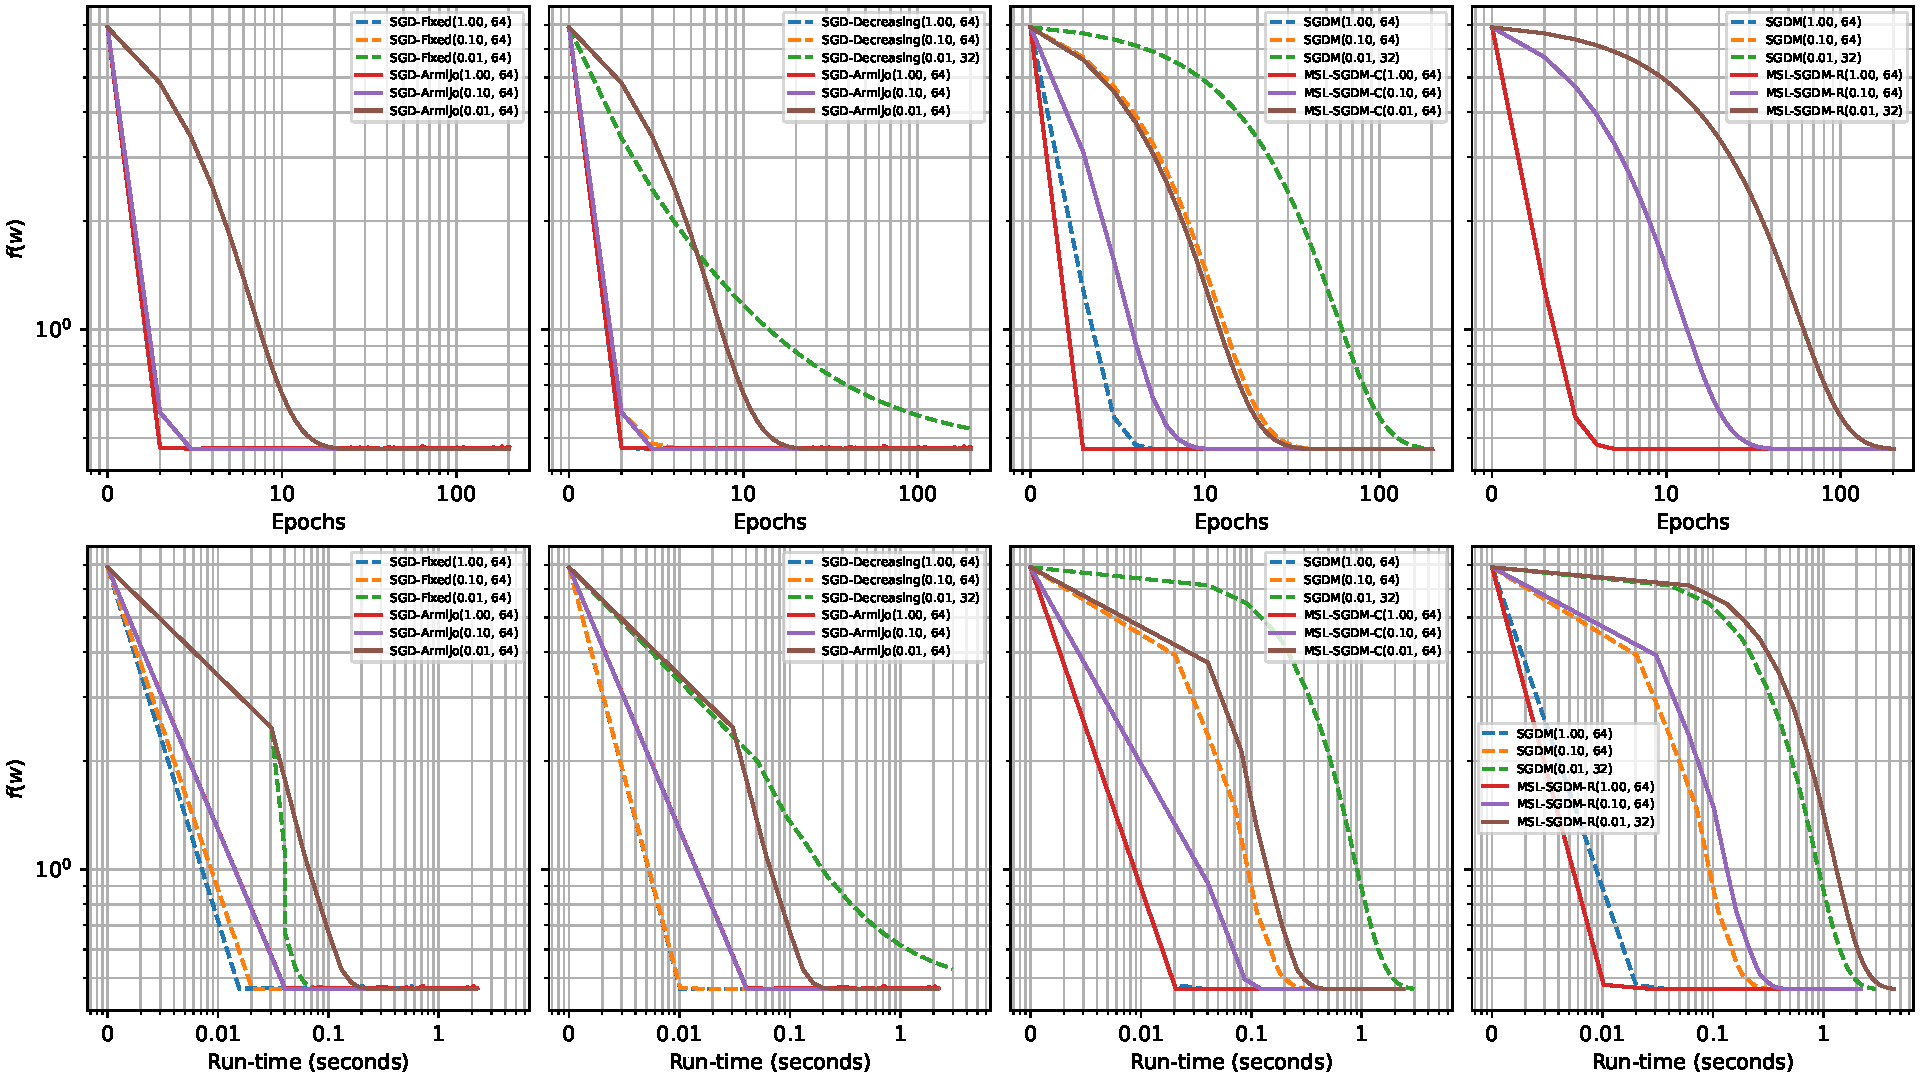
\includegraphics[width=\textwidth]{w1a-diagnostic}} \\
% w3a
\subfloat[][\emph{w3a dataset}\label{subfig:w3a-diagnostic}]%
{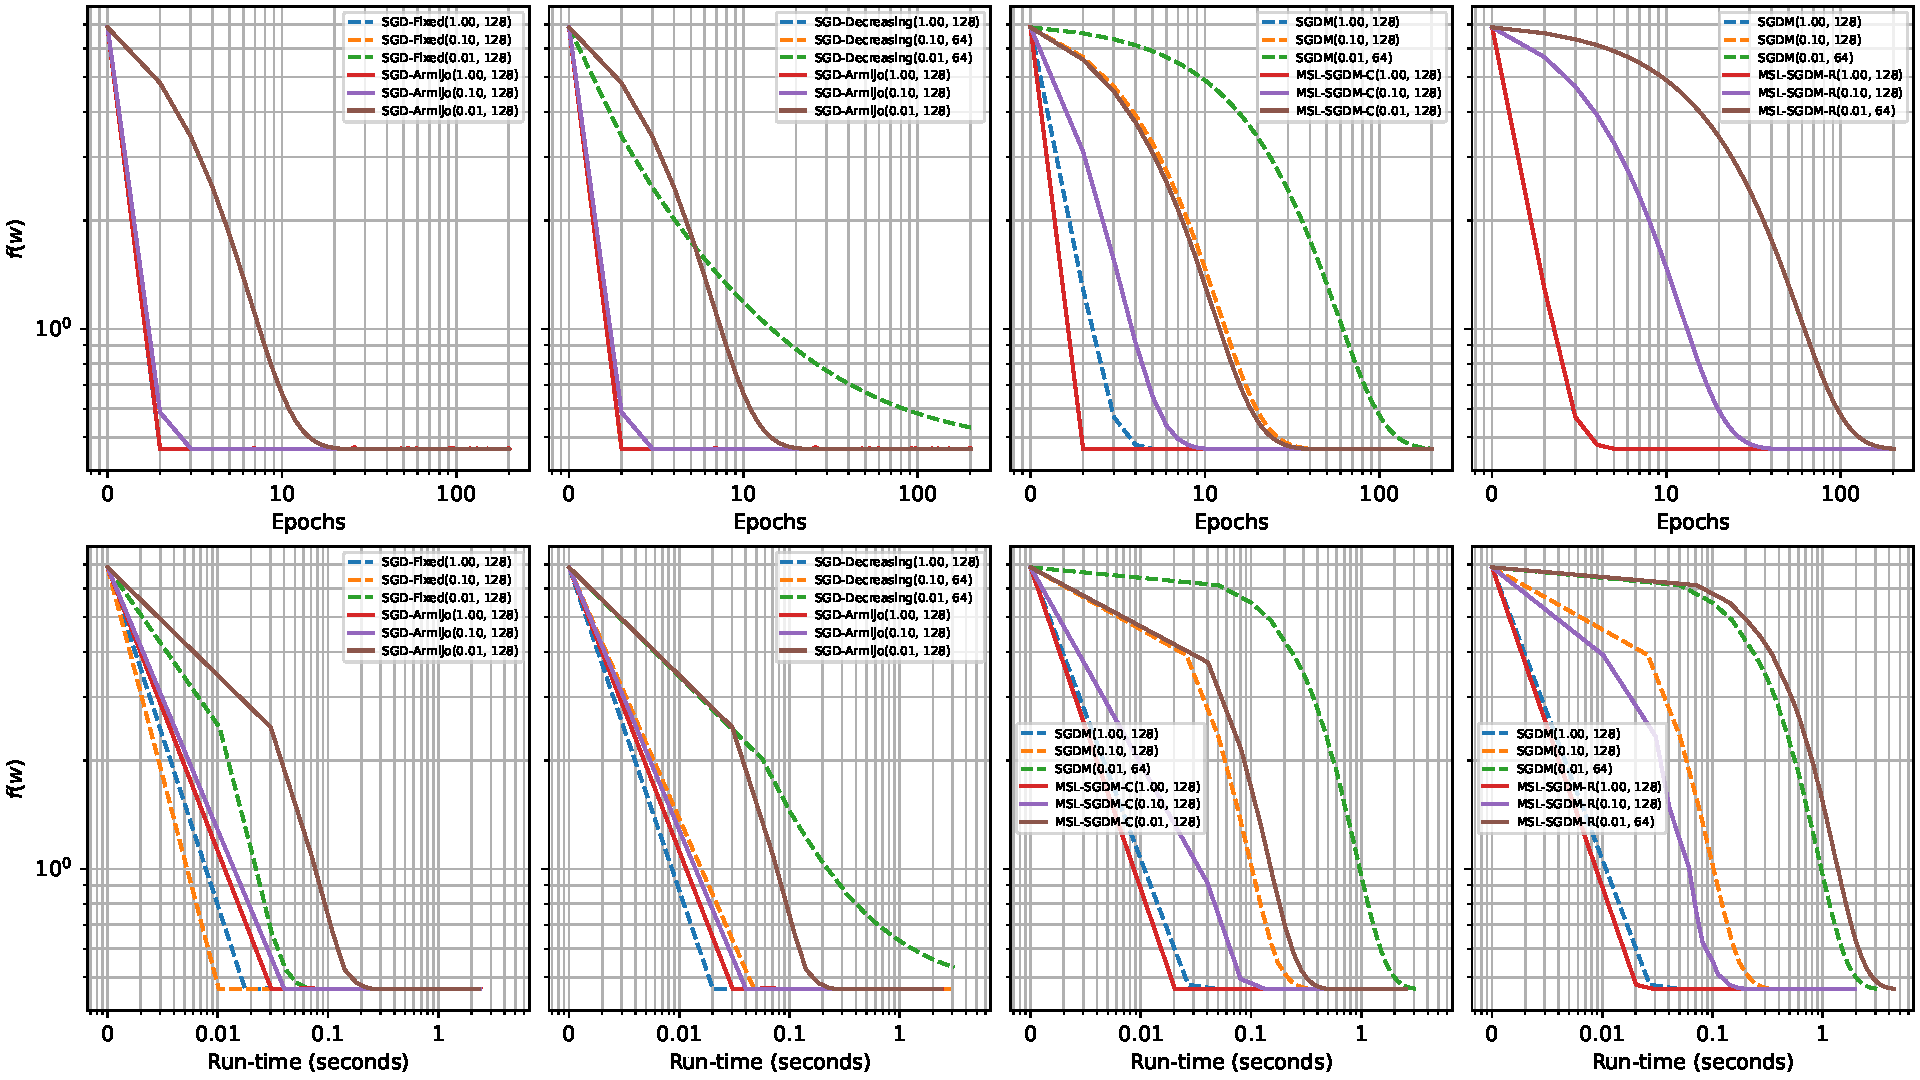
\includegraphics[width=\textwidth]{w3a-diagnostic}} \\
\caption[]{w1a and w3a datasets}
\label{fig:w1a-w3a}
\end{figure}

\begin{figure}
\centering
% Phishing
\subfloat[][\emph{Phishing dataset}\label{subfig:phish-diagnostic}]%
{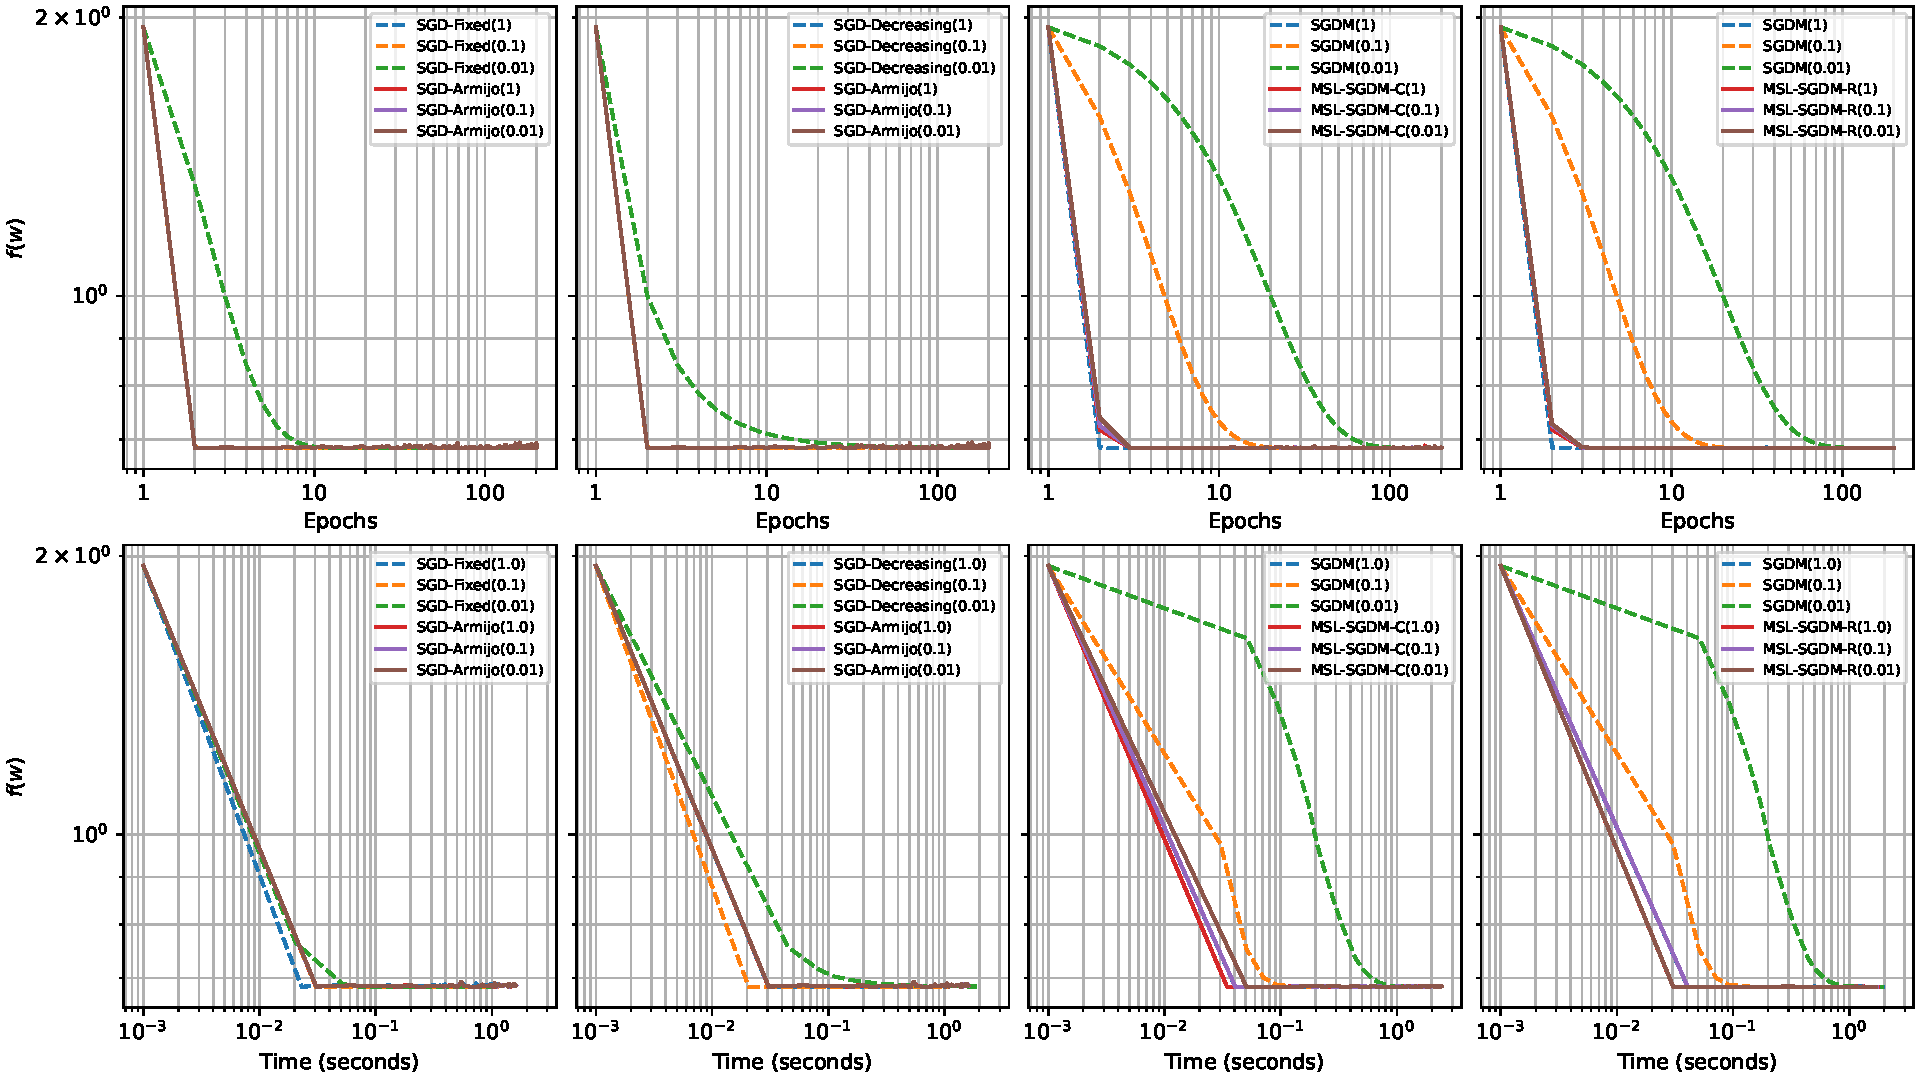
\includegraphics[width=\textwidth]{phish-diagnostic}} \\
% a2a
\subfloat[][\emph{a2a dataset}\label{subfig:a2a-diagnostic}]%
{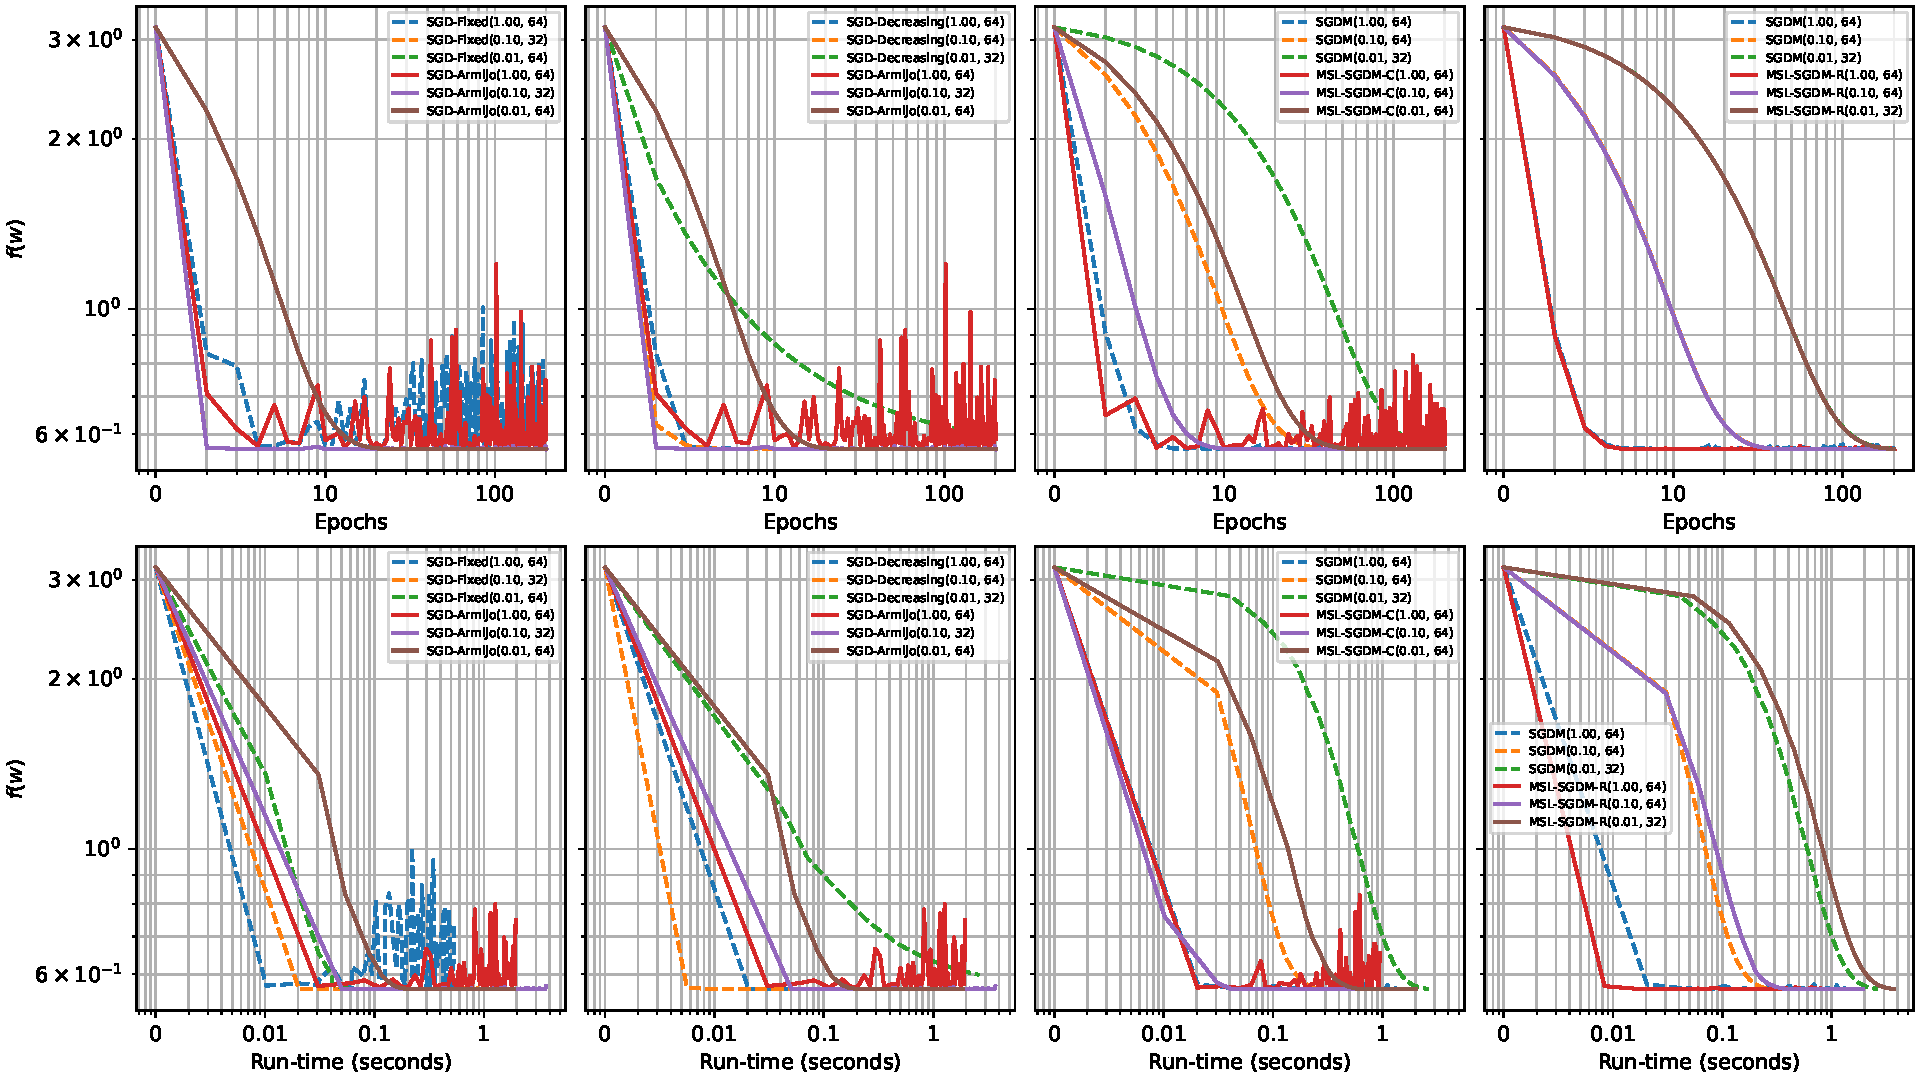
\includegraphics[width=\textwidth]{a2a-diagnostic}}
\caption[]{Phishing and a2a datasets}
\label{fig:phish-a2a}
\end{figure}

\begin{figure}
\centering
% mushrooms
\subfloat[][\emph{Mushrooms dataset}\label{subfig:mush-diagnostic}]%
{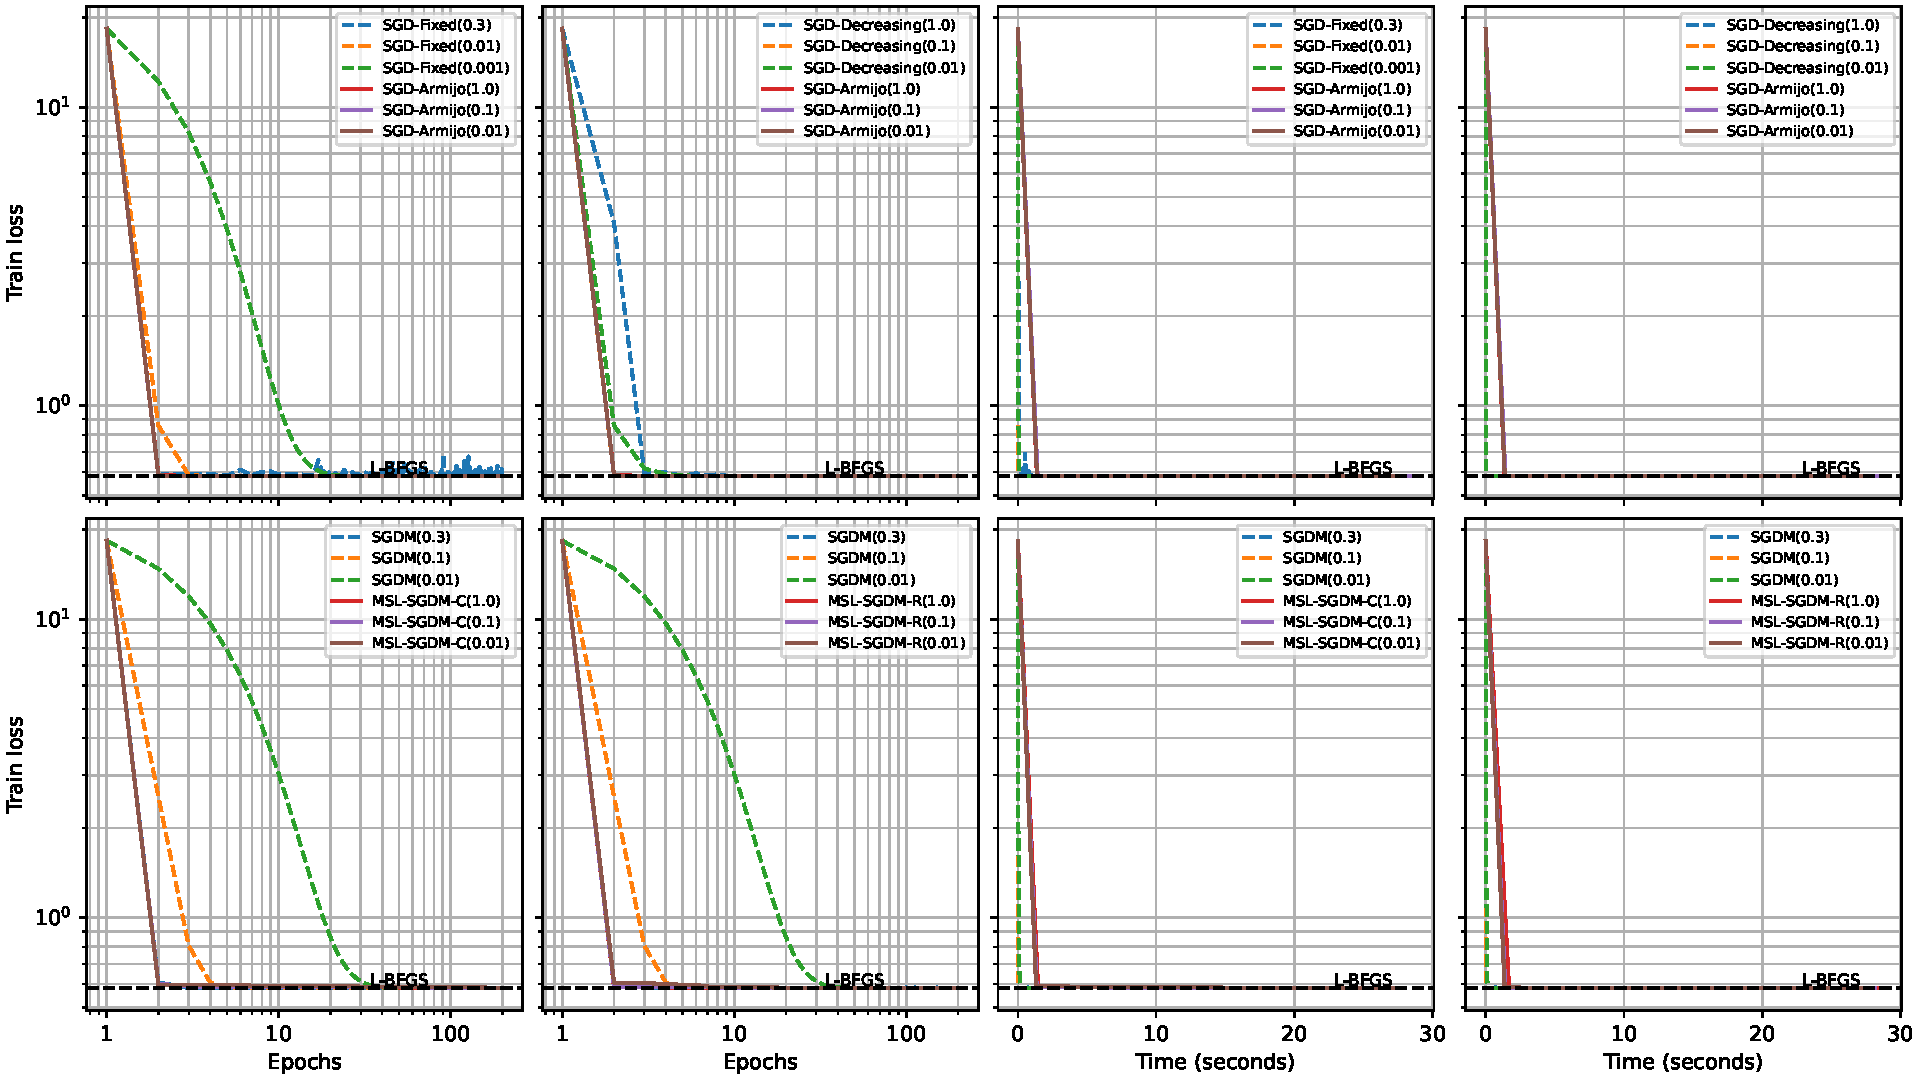
\includegraphics[width=\textwidth]{mush-diagnostic}} \\
% a4a
\subfloat[][\emph{a4a dataset}\label{subfig:a4a-diagnostic}]%
{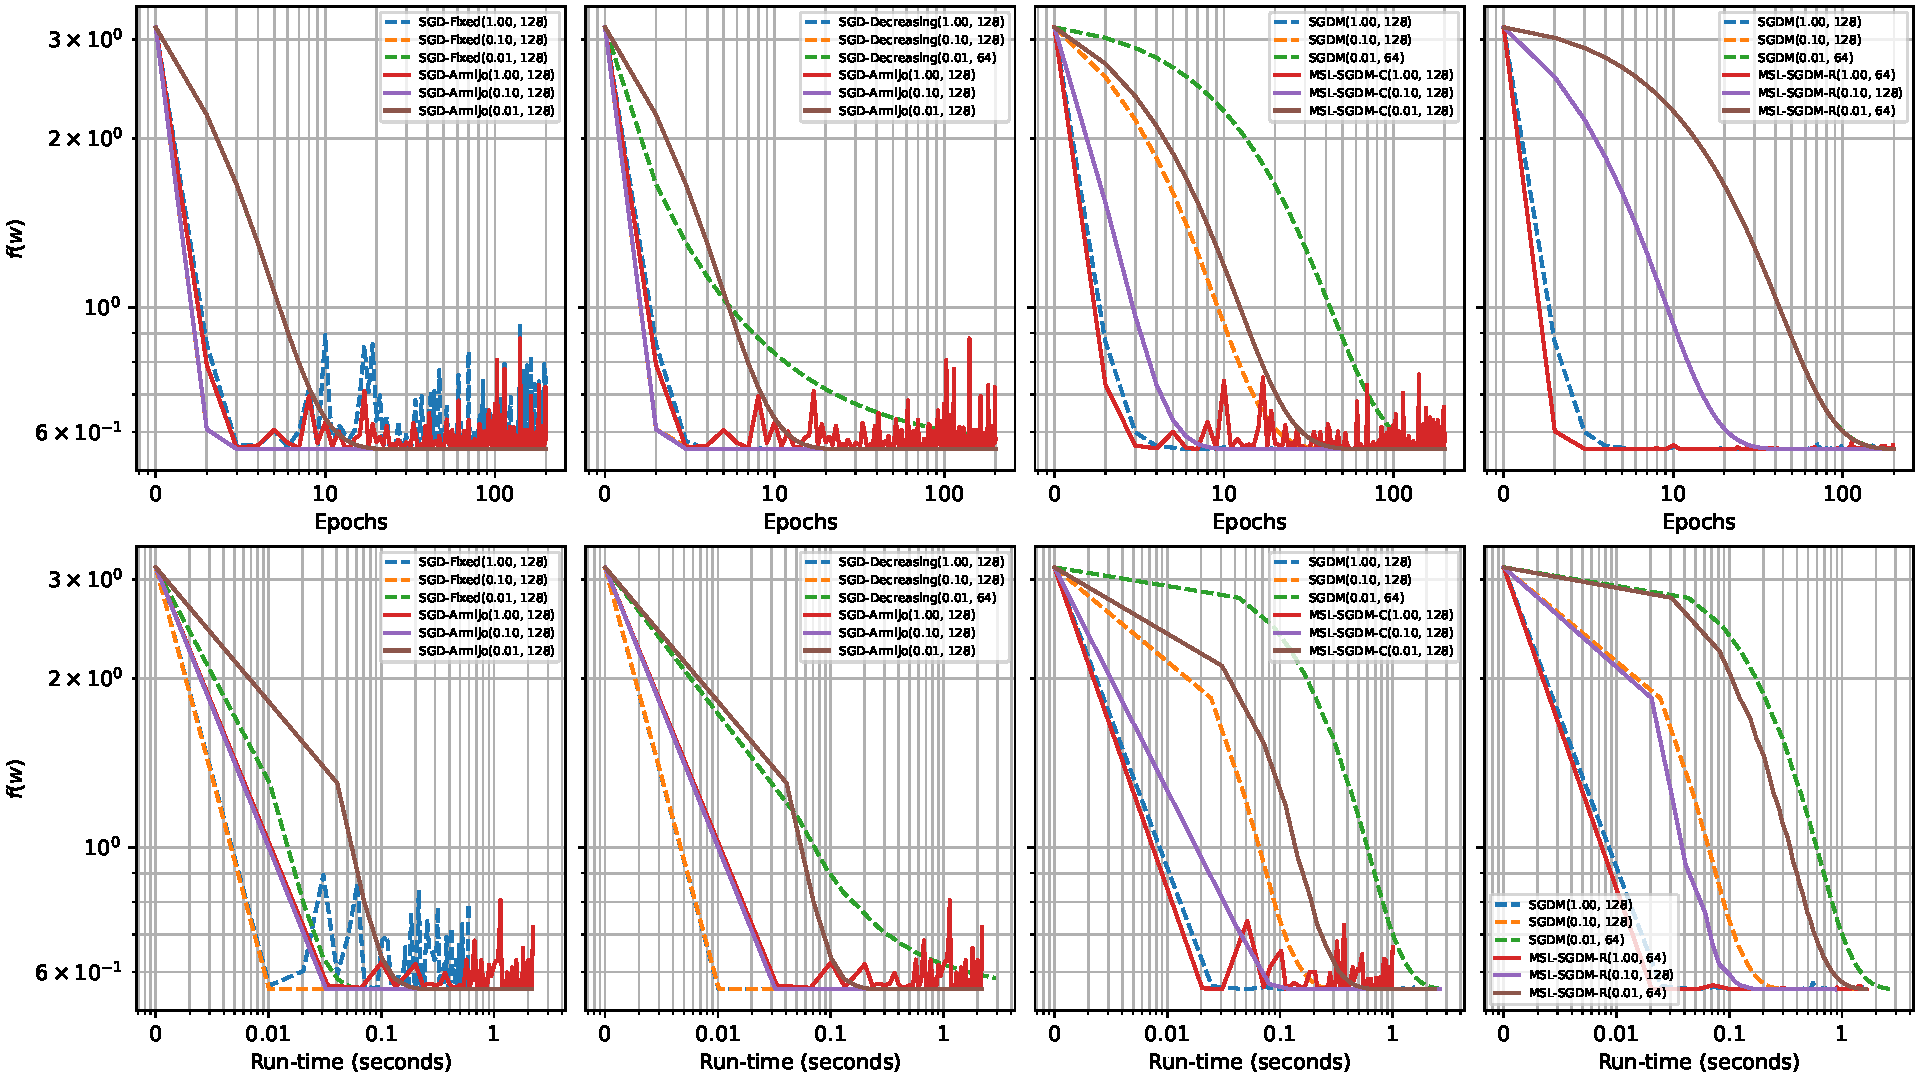
\includegraphics[width=\textwidth]{a4a-diagnostic}}
\caption[]{Mushrooms and a4a datasets}
\label{fig:mush-a4a}
\end{figure}

%\cleardoublepage
% ***************************************************** %
%\section{Mathematical background}
% ***************************************************** %

%\begin{defs}[Convex function]\label{def:conv_fun}
%	Let $S\subseteq\R^n$ be a convex set, a function $f\colon S\to\R$ is said to be convex if the hessian matrix is semi-positive-defined. If the hessian matrix is positive-defined, then the function is strictly convex.
%\end{defs}
%
%\begin{thm}[Weirstrass theorem]\label{thm:weirs}
%	Let $f\colon\R^n\to\R$ be a continuous function and $S\subseteq\R^n$ a compact set. Then function $f$ admits global minimum in $S$.
%\end{thm}
%
%\begin{cor}[Sufficient condition]\label{cor:weirs1}
%	If function $f\colon\R^n\to\R$ is a continuous and coercive function, then $f$ admits global minimum in $\R^n$.
%\end{cor}
%
%\begin{prop}[Coercivity of a quadratic function]
%	A quadratic function $\func(x)=\frac{1}{2}x^TQx-c^Tx$ is said to be coercive if and only if the symmetric matrix $Q\in\R^{n\times n}$ is positive-defined.
%\end{prop}
%
%\begin{prop}[Unique global minimum]\label{prop:min_unique}
%	Let $S\subseteq\R^n$ be a convex set, let $f\colon S\to\R$ be a strictly convex function. Then the global minimum, if exists, is unique.
%\end{prop}
%
%\begin{prop}[First order optimality condition]
%	$\bar{x}$ is a local minimum for $f\colon\R^n\to\R$ of class $f\in C^1(\R^n)$ if and only if $\nabla\func(\bar{x})=0$.
%\end{prop}
%
%\begin{prop}[Second order optimality condition]\label{prop:opt_second}
%	$\bar{x}\in\R^n$ is a local minimum for $f\colon\R^n\to\R$ of class $f\in C^2(\R^n)$ if and only if
%	\[\nabla\func(\bar{x})=0\quad\wedge\quad \nabla^2\func(\bar{x})\,\,\,\text{positive semi-definite}\]
%\end{prop}

% add definition of coercive function and proposition about compact sets?
% add gradient descent?
